\documentclass[a4paper, 12pt]{scrartcl}
\usepackage[utf8]{inputenc}
\usepackage[english]{babel}

\usepackage{hyperref}
\usepackage{graphicx}

\usepackage[left=2.5cm, right=2.5cm, top=2.0cm]{geometry}

\usepackage{setspace}
% \onehalfspacing

\usepackage[textsize=tiny]{todonotes}

\usepackage{acronym}
\newacro{ASIL}{Automotive Safety Integrity Level}
\acrodefplural{ASIL}{Automotive Safety Integrity Levels}
\newacro{DDS}{Data Distribution Service}
\newacro{ETCS}{European Train Control System}
\newacro{ERTMS}{European Rail Traffic Management System}
\newacro{ETCS OBU}{European Train Control System Onboard Unit}
\newacro{GNSS}{Global Navigation Satellite System}
\newacro{GNSSINS}[GNSS/INS]{Global Navigaion Satellite System/Inertial Navigation System}
\newacro{INS}{Inertial Navigation System}
\newacro{IOT}[IoT]{Internet of Things}
\acrodefplural{RBC}{Radio Block Centers}
\newacro{MA}{Movement Authority}
\acrodefplural{MA}{Movement Authorities}
\newacro{OMG}{Object Management Group}
\newacro{OS}{Operating System}
\newacro{QOS}[QoS]{Quality of Service}
\acrodefplural{QOS}[QoS]{Quality of Services}
\newacro{RBC}{Radio Block Center}
\newacro{SIL}{Safety Integrity Level}
\acrodefplural{SIL}{Safety Integrity Levels}
\newacro{SPS}[PLC]{Programmable Logic Controller}
\acrodefplural{SPS}[PLCs]{Programmable Logic Controllers}
\newacro{SSP}{Static Speed Profile}
\acrodefplural{SSP}{Static Speed Profiles}

% autoref with capital letter (from https://tex.stackexchange.com/a/40413)
\usepackage{catoptions}
\makeatletter
\def\figureautorefname{figure}
\def\tableautorefname{table}
\def\Autoref#1{%
  \begingroup
  \edef\reserved@a{\cpttrimspaces{#1}}%
  \ifcsndefTF{r@#1}{%
    \xaftercsname{\expandafter\testreftype\@fourthoffive}
      {r@\reserved@a}.\\{#1}%
  }{%
    \ref{#1}%
  }%
  \endgroup
}
\def\testreftype#1.#2\\#3{%
  \ifcsndefTF{#1autorefname}{%
    \def\reserved@a##1##2\@nil{%
      \uppercase{\def\ref@name{##1}}%
      \csn@edef{#1autorefname}{\ref@name##2}%
      \autoref{#3}%
    }%
    \reserved@a#1\@nil
  }{%
    \autoref{#3}%
  }%
}
\makeatother

\begin{document}


% Titel
\begin{center}
  \Huge{Master's Thesis Expos\'{e}}\\
  \large{\textsc{Hendrik Tjabben}}
\end{center}

% INTRODUCTION
% -------------------------------------------------------------------------------------

\section*{Introduction}
Embedded systems, which are deployed in safety-critical environments, must comply with certification requirements to demonstrate the systems' functional safety and integrity.
Nowadays, systems operating in safety-critical environments are demanded within various industries, including aerospace, medical, transportation and automotive applications.
In order to verify the system's safety, its compliance with the required assurance level is ensured during an approval process.
The conducted verification, validation and certification steps are very time- and cost-intensive.
Moreover, the approval process needs to be repeated every time the system is updated.

Modern safety-critical systems tend to distribute their computations to deal with the applied algorithm's increasing complexity and consequently expensive approval process.
However, work distribution introduces new challenges such as handling the communication overhead as well as dealing with node-, network and computation failures~\cite{DistributedSafety2020}.
In order to facilitate safe and real-time communication among participants, \ac{DDS}, which allows the definition of \ac{QOS}, can be used.
It features real-time support, safety, security and good interoperability with other middlewares~\cite{DistributedSafety2020}.
\ac{DDS} is already successfully applied in safety-critical environments such as underground railways where no constant communication can be guaranteed~\cite{DDSInURail}.
Redundant computation is the key technique for ensuring a system's reliability and safety, while also allowing failure correlation and self-recovery~\cite{TanenbaumSteen07}.
However, redundancy typically also complicates a system's approval process~\cite{ReliabilityThroughRedundancy}.

% AIM OF THE PROJECT
% -------------------------------------------------------------------------------------

\section*{Aim of the project}
Redundancy is often performed on homogenous nodes, which means that they use the same chip architecture and processing unit.
In the course of this master thesis, though, it is investigated how redundant computation on diverse nodes with different processing units can further improve a system's safety-level.
While distributed systems for safety mechanism, that build on top of \ac{DDS}, already exist in the automotive domain~\cite{DistributedSafety2020}, the system presented in this work focus the railway.
Therefore, the work done build on \ac{ETCS} and the CENELEC 50128:2011 standard for software in railway applications~\cite{BoulangerStandards}.
In addition, it will be determined whether there exists a suitable subset of \ac{DDS}, that is suitable to achieve the same results as in~\cite{DistributedSafety2020}, but with less expense and a reduced feature set.
Further, it is investigated to what extend a fine-tuning of \ac{DDS}, for example using participants' \ac{QOS} settings, can improve an application's safety, as proposed by Kugele et al.~\cite{KugeleDataCentricForAuto}.

For doing this, it is striven to cooperate with ADLINK~\footnote{\url{https://www.adlinktech.com/en/index.aspx}}, who build and maintain \ac{DDS} middlewares, such as Eclipse Cyclone DDS~\footnote{\url{https://github.com/eclipse-cyclonedds/cyclonedds}}, and corresponding tools.
The benefit of using a \ac{DDS} implementation by ADLINK is, that remaining certification and security issues are covered - as demanded by~\cite{KugeleDataCentricForAuto}.

For validating and demonstrating this approach, a distributed system architecture id build and assessed.
This system's special aspect is, that it should combine quality characteristics, such as modularity, control\-ler-level partitioning, and distributed diverse-redundant processing, with dynamic reconfiguration and data-driven designs.
The modular and distributed properties allow applications to be broken down in modules with distinct safety and integrity requirements.

In order to prove the approach, such a distributed system is build and validated against a core functionality of the \ac{ETCS OBU}.
Therefore, essential track-to-train messages from balises and \acp{RBC} are decoded, \acp{MA} and \acp{SSP} are calculated and the vehicle's speed is supervised.
The functional modules will be distributed across a modular system which is interconnected using the \ac{OMG} \ac{DDS} standard's publish-subscribe pattern.
Upon the test system, characteristics such as certifiability - with a focus modularity - maintainability and performance are examined.
Further, a high-level safety case analysis will be provided in order to identify functions that could be mapped to nodes with lower \acp{SIL}.

% EXPERIMENTAL SETUP
% -------------------------------------------------------------------------------------

\section*{Experimental Setup}

\begin{figure}
  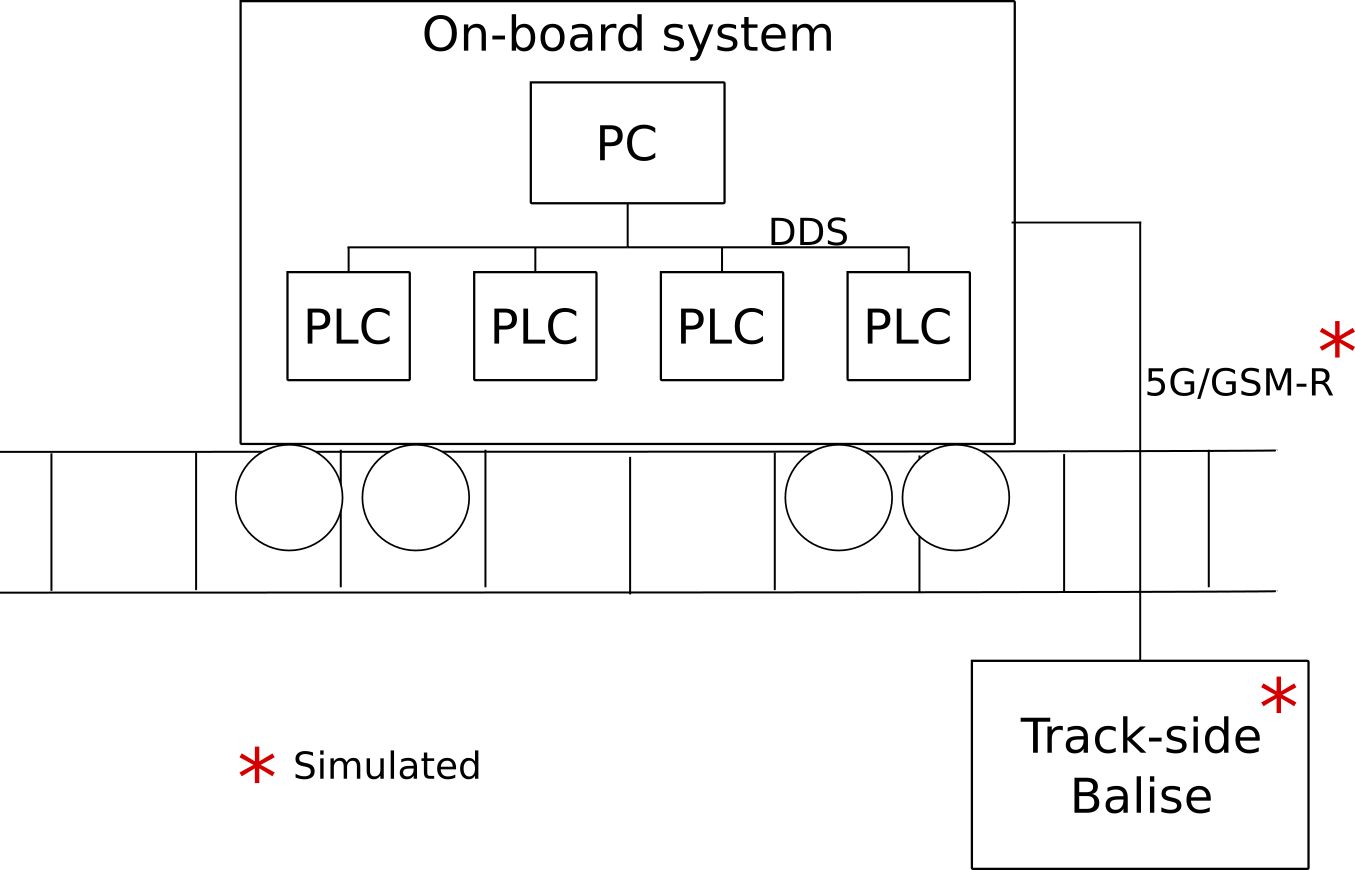
\includegraphics[width=\linewidth]{img/experimentalSetup.png}
  \caption{This work's experimental setup.}
  \label{fig:setup}
\end{figure}

The experimental setup is depicted in~\Autoref{fig:setup}.
It will comprise of a PC, four \acp{SPS}, an interconnect, a middleware layer running the \ac{DDS} standard and a simulation software.
The entire computation is done by the PC, which functions as the main computation unit but has no safety guarantees at all.
However, the \acp{SPS} feature a high \ac{SIL} \ac{OS} and are used for redudancy computation by only reprocessing the workload's safety-critical parts.
Synchronizing the \ac{SPS}'s results with the main PC supervises its work and wraps it into a safe envelope.
All \acp{SPS} are connected via an interconnect to the main PC.
By swapping out safety critical computations to the redundant working \acp{SPS} and sending data between individual components using the dependable real-time data exchange standard \ac{DDS}, the entire system can be raised to a high \ac{SIL}.

The simulation software imitates trackside balise as well as \ac{RBC} components and their corresponding data telegrams and messages, which are received and evaluated by the PC and the four \acp{SPS}.
In order to facilitate a realistic test environment, the balise and \ac{RBC} telegrams as well as the functional and operational principles are based on \ac{ETCS} Subset-026.

The simulation software should also be deployable to a lab vehicle's on-board system.
In that case, it will use positioning information based on \ac{GNSSINS} and odometry data of the lab vehicle in order to provide the system with virtual balise information.

% RELATED WORK
% -------------------------------------------------------------------------------------

\section*{Related Work}
Kugele et al. evaluate to what extend \ac{DDS} is feasible for automotive software~\cite{KugeleDataCentricForAuto}.
For answering this question, they implement an automotive service-oriented architecture and perform benchmark experiments upon this architecture.
For evaluating \ac{DDS}'s applicability in such a domain, Kugele et al. propose requirements and quality attributes for autonomous driving software.
The used list of requirements is composed by summarizing and adapting standards from the literature.
Their experiments are realized on a Ethernet topology with four Raspberry Pi 3 model B nodes and OpenDDS.
Results show that \ac{DDS} provides decent yet expandable availability and safety characteristics.
However, they also state that \ac{DDS} only covers automotive requirements when certain aspects, such as certification and security issues, are addressed.
\\

In their work, Bijlsma et al. extend the state-of-the-art E-Gas layered monitoring concept to handle faults in a distributed and redundant system~\cite{DistributedSafety2020}.
Upon their middleware, \ac{DDS} is applied to facilitate reliable communication among individual components with various \acp{ASIL}.
Besides functional data, diagnosis data is trasmitted using \ac{DDS} in order to detect faulty components.
\\

Jean-Louis Boulanger presents the 2011 version of the CENELEC 50128 standard and its implementations in his book~\cite{BoulangerStandards}.
CENELEC 50128 describes a software creation process for railway applications, as well as resources needed to achieve a set level of assurance.
Boulanger accentuates that the standard defines a context by which the safety of a software can be managed and thereby provides a guideline for safe software in the railway domain.

% WORK AND RISK ANALYSIS
% -------------------------------------------------------------------------------------

\section*{Work and Risk Analysis}
The project can be subdevided into four parts, namely a train and track simulator, a hardware setup, an on-board processing system as well as a testing and evaluation phase.
This work's main part is made up by the testing and evaluation phase, since this thesis' aim is to experiment and evaluate the system's configuration and characteristics.
The on-board processing system is comprised of data exchange with \ac{DDS}, decision making and redundancy computation.
It lays the foundation for the evaluation phase and is expected to take up the most time in this project.
Connecting the hardware is an essential part in this project but is unlikely to consume much time.
Simulating a train and track-side balises is choosen to be the show-case of this work.
Because of \ac{ETCS}'s complexity, building such a simulator from scratch is likely to take much resources.
It's preferred to either use existing simulators that provide the required packages or limit to very basic and time-periodic messages at first and postpone the implementation of a train simulation to the end of this project.
For evaluating the system, it is not mandatory that the analyzed messages conform to the \ac{ETCS} specification, so that adhering to \ac{ETCS} should not considered to be a main requirement of this project.

\bibliographystyle{plain}
\bibliography{bibtex}

\end{document}
